\section{The Proposed MT-DNN Model}
\label{sec:mt-dnn}
\begin{figure*}
	\centering
	\vspace{-1mm}
	% \adjustbox{trim={0.0\width} {0.71\height} {0.\width} {0.01\height},clip}
    {
	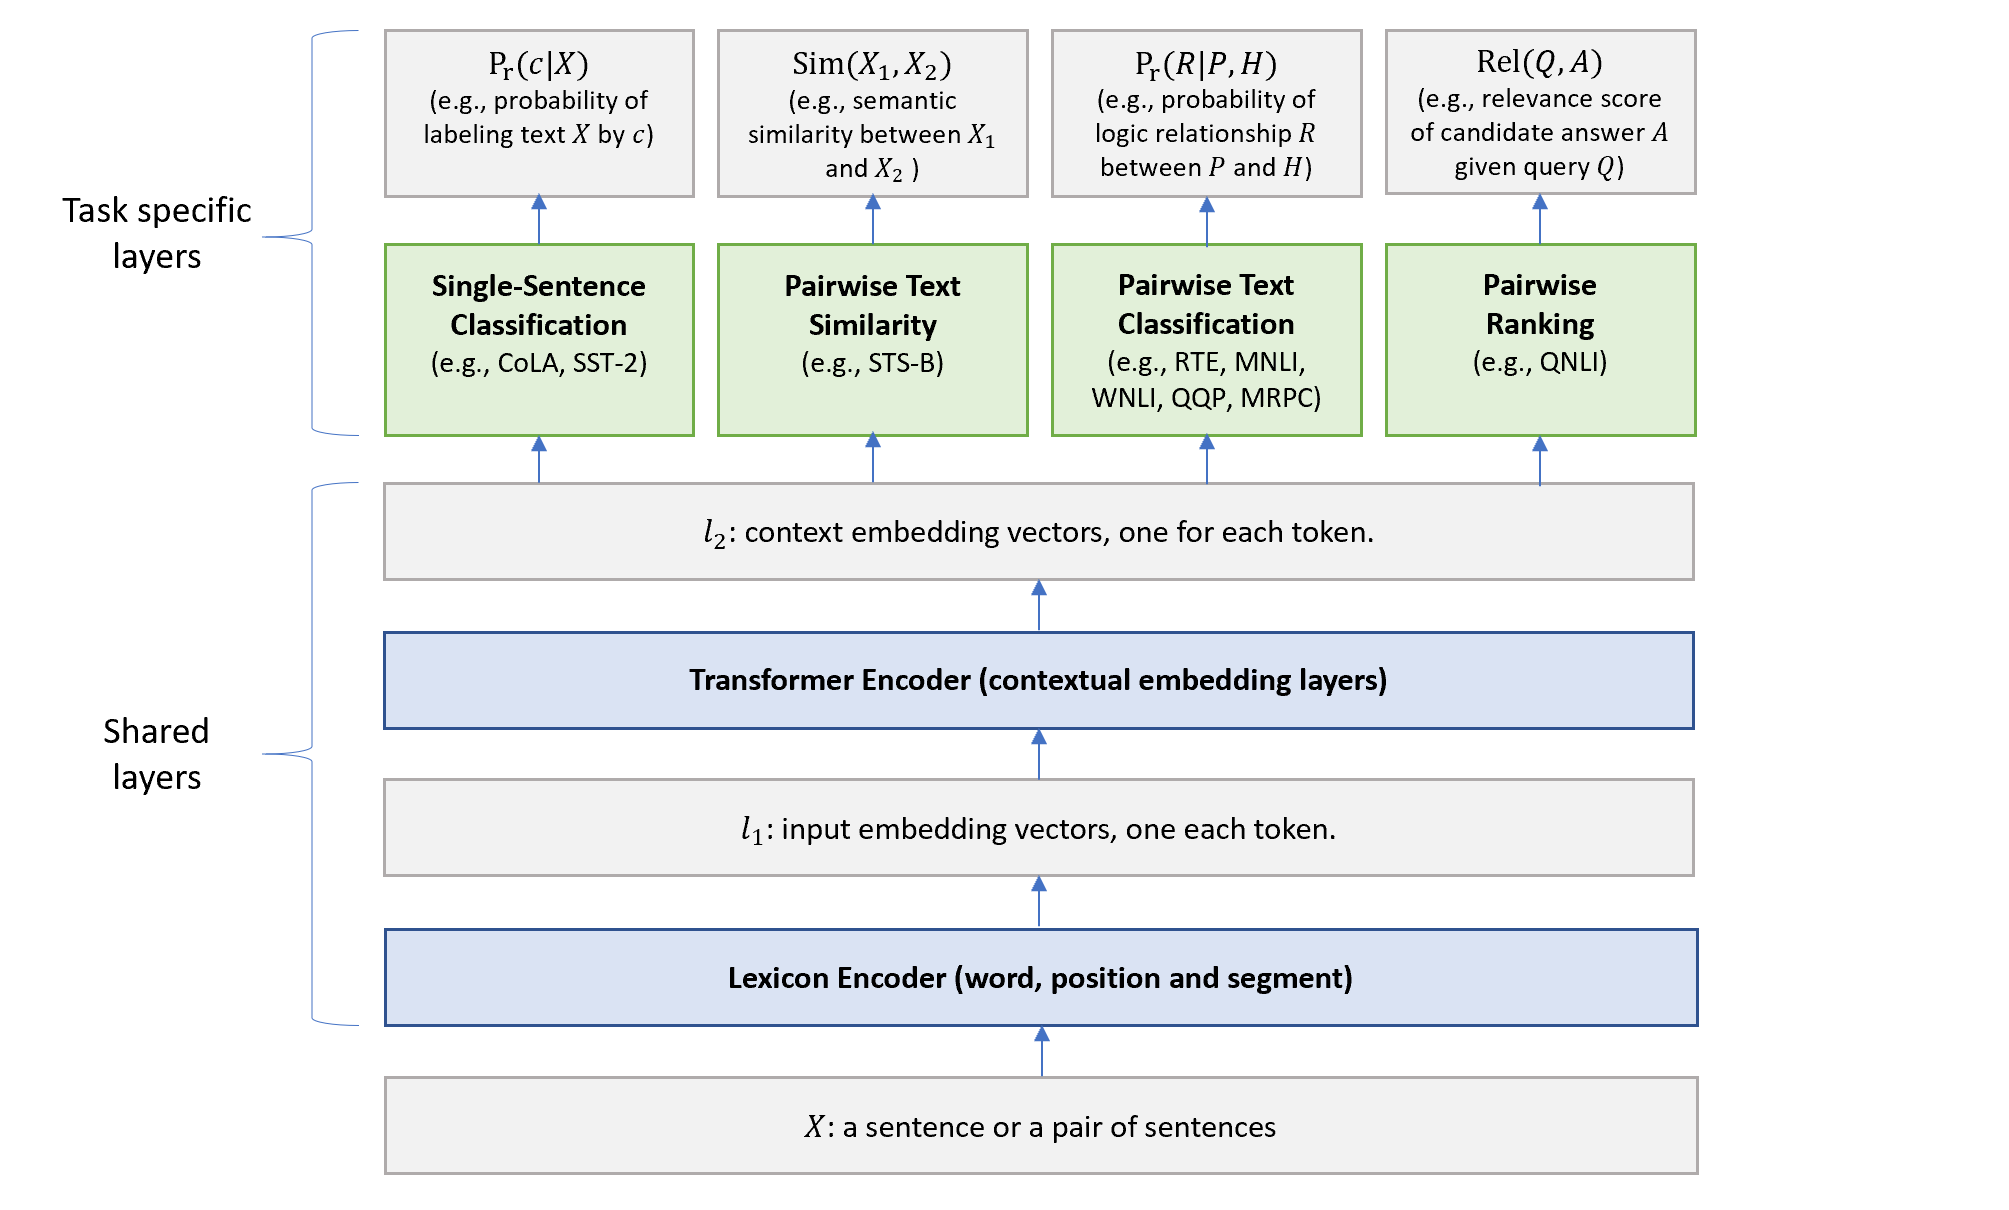
\includegraphics[width=0.92\textwidth]{fig/mt-dnn.png}
    }
	%\vspace{-2mm}
	\caption{Architecture of the MT-DNN model for representation learning. The lower layers are shared across all tasks while the top layers are task-specific. The input $X$ (either a sentence or a pair of sentences) is first represented as a sequence of embedding vectors, one for each word, in $l_1$. Then the Transformer encoder captures the contextual information for each word and generates the shared contextual embedding vectors in $l_2$. Finally, for each task, additional task-specific layers generate task-specific representations, followed by operations necessary for classification, similarity scoring, or relevance ranking.}
    %\vspace{-4mm}
	\label{fig:mt-dnn}
\end{figure*}


The architecture of the MT-DNN model is shown in Figure \ref{fig:mt-dnn}. The lower layers are shared across all tasks, while the top layers represent task-specific outputs. The input $X$, which is a word sequence (either a sentence or a pair of sentences packed together) is first represented as a sequence of embedding vectors, one for each word, in $l_1$. Then the transformer encoder captures the contextual information for each word via self-attention, and generates a sequence of contextual embeddings in $l_2$. This is the shared semantic representation that is trained by our multi-task objectives.  In what follows, we elaborate on the model in detail.

\paragraph{Lexicon Encoder ($l_1$):} 
The input $X=\{x_1,...,x_m\}$ is a sequence of tokens of length $m$. Following \citet{bert2018}, the first token $x_1$ is always the \texttt{[CLS]} token. 
If $X$ is packed by a sentence pair $(X_1, X_2)$, we separate the two sentences with a special token \texttt{[SEP]}. The lexicon encoder maps $X$ into a sequence of input embedding vectors, one for each token, constructed by summing the corresponding word, segment, and positional embeddings.

\paragraph{Transformer Encoder ($l_2$):}
We use a multi-layer bidirectional Transformer encoder \citep{vaswani2017attention} to map the input representation vectors ($l_1$) into a sequence of contextual embedding vectors 
$\mathbf{C} \in \mathbb{R}^{d \times m}$. 
This is the shared representation across different tasks. Unlike the BERT model \citep{bert2018} that learns the representation via pre-training,
% and adapts it to each individual task via fine-tuning, 
MT-DNN learns the representation using multi-task objectives, in addition to pre-training.

Below, we will describe the task specific layers using the NLU tasks in GLUE as examples, although in practice we can incorporate arbitrary natural language tasks such as text generation where the output layers are implemented as a neural decoder.

\paragraph{Single-Sentence Classification Output:}
Suppose that $\mathbf{x}$ is the contextual embedding ($l_2$) of the token \texttt{[CLS]}, which can be viewed as the semantic representation of input sentence $X$. Take the SST-2 task as an example. The probability that $X$ is labeled as class $c$ (i.e., the sentiment) is predicted by a logistic regression with softmax:
\begin{equation}
P_r(c|X)= \text{softmax} (\mathbf{W}_{SST}^\top \cdot \mathbf{x}),
\label{eqn:single-sent-classification}
\end{equation}
where $\mathbf{W}_{SST}$ is the task-specific parameter matrix.

\paragraph{Text Similarity Output:}
Take the STS-B task as an example. Suppose that $\mathbf{x}$ is the contextual embedding ($l_2$) of \texttt{[CLS]} which can be viewed as the semantic representation of the input sentence pair $(X_1, X_2)$. We introduce a task-specific parameter vector $\mathbf{w}_{STS}$ to compute the similarity score as: 
\begin{equation}
\text{Sim} (X_1, X_2)= \mathbf{w}_{STS}^\top \cdot \mathbf{x},
\label{eqn:text-sim}
\end{equation}
where $\text{Sim} (X_1, X_2)$ is a real value of the range (-$\infty$, $\infty$).

%where $g(z)= \frac{1}{1+\exp{(-z)}}$ is a sigmoid function that maps the score to a real value of the range $[0, 1]$.

\paragraph{Pairwise Text Classification Output:}
Take natural language inference (NLI) as an example. The NLI task defined here involves a premise $P = (p_1,...,p_m)$ of $m$ words and a hypothesis $H = (h_1,..., h_n)$  of $n$ words, and aims to find a logical relationship $R$ between $P$ and $H$. The design of the output module follows the answer module of the stochastic answer network (SAN) \citep{liu2018san4nli}, a state-of-the-art neural NLI model. SAN's answer module uses multi-step reasoning. Rather than directly predicting the entailment given the input, it maintains a state and iteratively refines its predictions.

The SAN answer module works as follows. We first construct the working memory of premise $P$ by concatenating the contextual embeddings of the words in $P$, which are the output of the transformer encoder, denoted as $\mathbf{M}^p \in \mathbb{R}^{d \times m}$, and similarly the working memory of hypothesis $H$, denoted as $\mathbf{M}^h \in \mathbb{R}^{d \times n}$. 
Then, we perform $K$-step reasoning on the memory to output the relation label, where $K$ is a hyperparameter.
At the beginning,  the initial state $\mathbf{s}^0$ is the summary of $\mathbf{M}^h$: 
$\mathbf{s}^0 = \sum_j \alpha_j\mathbf{M}_j^h$, 
where $\alpha_j = \frac {\exp(\mathbf{w}_1^\top \cdot \mathbf{M}_j^h)} {\sum_i \exp(\mathbf{w}_1^\top \cdot \mathbf{M}_i^h)}$. 
At time step $k$ in the range of $\{1,2,…,K-1\}$, the state is defined by 
$\mathbf{s}^k = \text{GRU} (\mathbf{s}^{k-1}, \mathbf{x}^k)$. 
Here, $\mathbf{x}^k$ is computed from the previous state $\mathbf{s}^{k-1}$ and memory $\mathbf{M}^p$: $\mathbf{x}^k = \sum_j \beta_j\mathbf{M}_j^p$ and $\beta_j = \text{softmax} (\mathbf{s}^{k-1} \mathbf{W}_2^\top \mathbf{M}^p )$. 
A one-layer classifier is used to determine the relation at each step $k$:
\begin{equation}
P_r^k = \text{softmax} (\mathbf{W}_3^\top [\mathbf{s}^k ; \mathbf{x}^k ; |\mathbf{s}^k - \mathbf{x}^k|; \mathbf{s}^k \cdot \mathbf{x}^k ]).
\label{eqn:pairwise-text-classification}
\end{equation}
 
At last, we utilize all of the $K$ outputs by averaging the scores:
\begin{equation}
P_r = \text{avg} ([P_r^0, P_r^1, ..., P_r^{K-1}]).
\label{eqn:pairwise-text-classification-avg}
\end{equation}

Each $P_r$ is a probability distribution over all the relations $R \in \mathcal{R}$. 
During training, we apply \emph{stochastic prediction dropout} \citep{liu2018san} before the above averaging operation. 
During decoding, we average all outputs to improve robustness.

\paragraph{Relevance Ranking Output:}
Take QNLI as an example. Suppose that $\mathbf{x}$ is the contextual embedding vector of \texttt{[CLS]} which is the semantic representation of a pair of question and its candidate answer $(Q, A)$. 
%We introduce a task-specific parameter vector $\mathbf{w}_{QNLI}$ to compute the relevance score as: 
We compute the relevance score as: 
\begin{equation}
\text{Rel} (Q, A)= g (\mathbf{w}_{QNLI}^\top \cdot \mathbf{x}),
\label{eqn:rel-score}
\end{equation}
For a given $Q$, we rank all of its candidate answers based on their relevance scores computed using Equation \ref{eqn:rel-score}.

\subsection{The Training Procedure}

The training procedure of MT-DNN consists of two stages: pretraining and multi-task learning. The pretraining stage follows that of the BERT model \citep{bert2018}. The parameters of the lexicon encoder and Transformer encoder are learned using two unsupervised prediction tasks: masked language modeling and next sentence prediction.\footnote{In this study we use the pre-trained BERT models released by the authors.}

In the multi-task learning stage, we use mini-batch based stochastic gradient descent (SGD) to learn the parameters of our model (i.e., the parameters of all shared layers and task-specific layers) as shown in Algorithm \ref{algo:mtdnn}.  In each epoch, a mini-batch $b_t$ is selected(e.g., among all 9 GLUE tasks), and the model is updated according to the task-specific objective for the task $t$. This approximately optimizes the sum of all multi-task objectives. 
\begin{algorithm}[ht!]
 \SetAlgoLined
Initialize model parameters $\Theta$ randomly.  \\
Pre-train the shared layers (i.e., the lexicon encoder and the transformer encoder). \\
Set the max number of epoch: $epoch_{max}$.
\textit{//Prepare the data for $T$ tasks.}\\
\For{$t$ in $1,2,...,T$ }
{
    Pack the dataset $t$ into mini-batch: $D_t$.
}

 \For{$epoch$ in $1,2,...,epoch_{max}$}{
     1. Merge all the datasets: $D =D_1 \cup D_2 ... \cup D_T$ \\
     2. Shuffle $D$ \\
     \For{$b_t$ in D}{
        \textit{//$b_t$ is a mini-batch of task $t$.} \\
        % Note that if the task $t$ is a classification task, Equation~\ref{eqn:cross-entropy-loss} is used; if the task $t$ is a regression task, Equation~\ref{eqn:msq-loss} is used; and if the task $t$ is a ranking task, Eq~\ref{eqn:ranking-loss} is used.}
     3. Compute loss : $L(\Theta)$ \\
        \hspace{0.3cm} $L(\Theta)=$ Eq.~\ref{eqn:cross-entropy-loss} for classification \\
        \hspace{0.3cm} $L(\Theta)=$ Eq.~\ref{eqn:msq-loss} for regression \\
        \hspace{0.3cm} $L(\Theta)=$ Eq.~\ref{eqn:ranking-loss} for ranking \\
     4. Compute gradient: $\nabla(\Theta)$ \\
     5. Update model: $\Theta = \Theta - \epsilon \nabla(\Theta)$ \\
     }
 }
 \caption{\label{algo:mtdnn} Training a MT-DNN model.}
%\vspace{-0.3cm} 
 % \algorithmfootnote{Note that $\Theta$ denotes the model parameters and T is the number of tasks.}
\end{algorithm} %\vspace{-0.2cm} 

% \begin{algorithm}[ht!]
%  \SetAlgoLined
% Initialize model parameters $\Theta$ randomly  \\
% %Set M \quad\textit{//the number of updates for the shared layer} \\
% %\textit{Counter} = 0\\
%  \For{$iteration$ in $0 ... \infty$}{
%  	 %1. \textit{Counter} += 1\\
%      1. Pick a task $t$ randomly \\
%      2. Pick sample(s) from task $t$, i.e., \\
%      \hspace{0.4cm}$(Q,C=\{0,1\})$ for classification \\
%      \hspace{0.4cm}$(Q, D)$ for ranking\\
%      3. Compute loss: $L(\Theta)$, i.e.,\\
%      \hspace{0.4cm} the \textit{cross-entropy} for classification \\
%      \hspace{0.4cm} the ranking loss for ranking\cite{learning-to-rank2005burges}\\

%      4. Compute gradient: $\nabla(\Theta)$ \\
%      5. Update model: $\Theta = \Theta - \epsilon \nabla(\Theta)$ \quad\textit{}
%      % \eIf{Counter $<$ M}{
%   	 %5. Update model: $\Theta = \Theta - \epsilon \nabla(\Theta)$ \quad\textit{//update both $\Theta^s$ and $\Theta^t$} \\
%   %}{
%   	% 6. Update model: $\Theta^t = \Theta^t - \epsilon \nabla(\Theta^t)$ 
%   %}
%  }
%  \caption{\label{algo:mtdnn} Training a MT-DNN model.}
%  \algorithmfootnote{Note that $\Theta$ denotes the model parameters. \textcolor{red}{TODO: update alg based on task defination.}}
% \end{algorithm}

For the classification tasks (i.e., single-sentence or pairwise text classification), we use the cross-entropy loss as the objective:
\begin{equation}
-\sum_c \mathbbm{1}(X,c) \log(P_r(c|X)),
\label{eqn:cross-entropy-loss}
\end{equation}
where $\mathbbm{1}(X,c)$ is the binary indicator (0 or 1) if class label $c$ is the correct classification for $X$, and $P_r(.)$ is defined by e.g., Equation \ref{eqn:single-sent-classification} or \ref{eqn:pairwise-text-classification-avg}.

For the text similarity tasks, such as STS-B, where each sentence pair is annotated with a real-valued score $y$, we use the mean squared error as the objective:
\begin{equation}
(y - \text{Sim}(X_1, X_2))^2,
\label{eqn:msq-loss}
\end{equation}
where $\text{Sim}(.)$ is defined by Equation \ref{eqn:text-sim}.

The objective for the relevance ranking tasks follows the pairwise learning-to-rank paradigm \citep{learning-to-rank2005burges,huang2013dssm}. Take QNLI as an example. Given a query $Q$, we obtain a list of candidate answers $\mathcal{A}$ which contains a positive example $A^+$ that includes the correct answer, and $|\mathcal{A}|-1$ negative examples. We then minimize the negative log likelihood of the positive example given queries across the training data
\begin{equation}
-\sum_{(Q,A^+)} P_r(A^+ | Q),
\label{eqn:ranking-loss}
\end{equation}
%where the probability of a given answer $A^+$ is computed as
\begin{equation}
P_r(A^+ | Q) = \frac{\exp(\gamma \text{Rel}(Q,A^+))}{\sum_{A^{'} \in \mathcal{A}} \exp(\gamma \text{Rel}(Q,A^{'}))},
\label{eqn:ranking-prob}
\end{equation}
where $\text{Rel}(.)$ is defined by Equation \ref{eqn:rel-score} and $\gamma$ is a tuning factor determined on held-out data. In our experiment, we simply set $\gamma$ to 1.

%Similar to the BERT model, we can adapt the trained MT-DNN to any new task via fine-tuning on task-specific data. 
%After the multi-task training, we could directly use the multi-task model to perform prediction on each task. Alternative, this model can be further fine-tuned using task-specific data for each individual task.  The detailed empirical study of these two approaches will be provided in Section \ref{sec:exp}.
